\documentclass[12pt,a4paper]{article}
\usepackage[utf8]{inputenc}
\usepackage[croatian]{babel} % For Croatian 
\usepackage[T1]{fontenc} % Better hyphenation for wrods with digraphs čćžšđ
\usepackage{graphicx}
\usepackage{color}
\usepackage{float} % For manualy figure postioning
\usepackage{listings} % Support for .txt listings w/o begin{verbatim}
\usepackage[usenames,dvipsnames]{xcolor} % Enabling more defined colors
\usepackage{datetime}
\usepackage{tocloft} % For Toc with dots
\usepackage[left=3cm,top=2.5cm,right=2.5cm,bottom=2.5cm]{geometry} 
\usepackage{fancyhdr} % For fancy headers and footers
\usepackage[nottoc]{tocbibind} % For adding Bilbiography in TOC
\usepackage{amsmath}
% ---------------------------------------------------------------------------
% Fancy header definition
% ---------------------------------------------------------------------------
\setlength{\headheight}{15.2pt}
\pagestyle{fancy}
\fancyhf{}
\rhead{ \bfseries \color{MidnightBlue}  }
\renewcommand{\sectionmark}[1]{\markright{#1}{}} % Section mark to small case
\renewcommand{\subsectionmark}[1]{\markright{#1}{}} % Section mark to small case
\lhead{\sectionmark}
\lhead{\rightmark}
\rfoot{\thepage}
\linespread{1.3}

\renewcommand\lstlistingname{Unos}
\renewcommand\lstlistlistingname{Unos}

\lstnewenvironment{code}[1][]%
  {\minipage{\linewidth} 
   \lstset{
        basicstyle=\ttfamily\footnotesize,
        language=Matlab,
        captionpos=b,
        keywordstyle=\color{blue},
        frame=single,
        #1}}
  {\endminipage}

\definecolor{mygreen}{rgb}{0,0.6,0}
\definecolor{mygray}{rgb}{0.5,0.5,0.5}
\definecolor{mymauve}{rgb}{0.58,0,0.82}

\lstset{ %
  backgroundcolor=\color{white},   % choose the background color; you must add \usepackage{color} or \usepackage{xcolor}
  basicstyle=\footnotesize\ttfamily,% the size of the fonts that are used for the code
  breakatwhitespace=false,         % sets if automatic breaks should only happen at whitespace
  breaklines=true,                 % sets automatic line breaking
  captionpos=b,                    % sets the caption-position to bottom
  commentstyle=\color{mygreen},    % comment style
  deletekeywords={...},            % if you want to delete keywords from the given language
  escapeinside={\%*}{*)},          % if you want to add LaTeX within your code
  extendedchars=true,              % lets you use non-ASCII characters; for 8-bits encodings only, does not work with UTF-8
  frame=single,                    % adds a frame around the code
  keepspaces=true,                 % keeps spaces in text, useful for keeping indentation of code (possibly needs columns=flexible)
  keywordstyle=\color{blue},       % keyword style
  language=C,                      % the language of the code
  morekeywords={*,...},            % if you want to add more keywords to the set
  numbers=left,                    % where to put the line-numbers; possible values are (none, left, right)
  numbersep=5pt,                   % how far the line-numbers are from the code
  numberstyle=\tiny\color{mygray}, % the style that is used for the line-numbers
  rulecolor=\color{black},         % if not set, the frame-color may be changed on line-breaks within not-black text (e.g. comments (green here))
  showspaces=false,                % show spaces everywhere adding particular underscores; it overrides 'showstringspaces'
  showstringspaces=false,          % underline spaces within strings only
  showtabs=false,                  % show tabs within strings adding particular underscores
  stepnumber=2,                    % the step between two line-numbers. If it's 1, each line will be numbered
  stringstyle=\color{mymauve},     % string literal style
  tabsize=2,                       % sets default tabsize to 2 spaces
  title=\lstname                   % show the filename of files included with \lstinputlisting; also try caption instead of title
}

\begin{document}

% Section, figure, table numbering
\renewcommand{\thesection}{\arabic{section}.}
\renewcommand{\thesubsection}{\arabic{section}.\arabic{subsection}}
\renewcommand{\thefigure}{\arabic{section}.\arabic{figure}} 
\renewcommand{\thetable}{\arabic{section}.\arabic{table}}

\newpage
\begin{titlepage}
\begin{center}
% Definition of HRule command
\newcommand{\HRule}[1]{\rule{\linewidth}{#1}}

\textsc{Sveučilište Josipa Jurja Strossmayera u Osijeku}\\[0.2cm]
\textbf{\textsc{Elektrotehnički fakultet Osijek}}\\[4.5cm]
%\includegraphics[scale=0.35]{graphs/etfos_logo.eps}\\[2cm]    

% Title
%\HRule{1.5pt} \\[0.2cm]

{\large \bfseries \textsc{Svalina Marijan, D287} \\ [1 cm] } 
{\LARGE \bfseries \color{MidnightBlue} 
ROBOTSKI VID \\ laboratorijske vježbe \\ [0.5cm] }
{\large \bfseries izvještaj} \\ [0.2cm]

%\HRule{2pt} 

\vfill
% Author 

\begin{minipage}{0.4\textwidth}
\begin{center} \large
Osijek, \today \\
\end{center}


\end{minipage}
\end{center}
\end{titlepage}
\newpage
% Toc  
\renewcommand{\cftsecleader}{\cftdotfill{\cftdotsep}}
\tableofcontents 
% Removing page numbering from TOC
\thispagestyle{empty}

\newpage
\setcounter{page}{1}


\setcounter{figure}{0}
\section{Vježba 1: Uvod u OpenCV i podešavanje radne okoline}

\subsection{Cilj vježbe}
Upoznati se s bibliotekom OpenCV. Podesiti i proučiti alate za
prevođenje i izvršavanje izvornog koda. Napisati jednostavan program za
određivanje rubova na slici pomoću \emph{Canny-evog} detektora rubova.
Proširiti program funkcijom rezanja slike i dodati mogućnosti učitavnja
videa.\\

\subsection{Kratak info o OpenCV-u}

OpenCV (\emph{Open Source Computer Vision Library})je biblioteka C i C++
funkcija koje se često upotrebljavaju u računalnom vidu. Početno
razvijena od strane Intel-a, a trenutno ju održavaju Willow Garage i
Itseez.  Slobodna je za upotrebu pod uvijetima BSD licence. Biblioteka
se izvodi na svim većim platformama. Fokusira se na obradu slike u
stvarnom vremenu.

\subsection{Radna okolina}

\begin{description}
  \item[OS:] Ubuntu 12.04
  \item[Biblioteka:] OpenCV 2.4.6
  \item[Prevodioc:] GCC 4.6.3 
  \item[Ostalo:] pkg-config 0.26
\end{description}

Ubuntu 12.04 je izabran zbog stabilnosti, jednostavnog podešavanja i 
dostupnosti velike količine već priprmljenih programskih paketa.
OpenCV 2.4.6 je zadnja stabilna verzija u trenutnku pisanja. Odabrana
je jer se razvoj aplikacija odrađivao na više računala s različitim 
GNU/Linux distribucijama te zbog dostupnosti najnovih funkicija.
GCC 4.6.3 je zadna verzija koja dolazi s Ubuntu 12.04 distribucijom.
pkg-config alat je korišten jer on automatski izlista potrebne
opencv biblioteke i datoteke zaglavlja prevodiocu. 
\\

\begin{lstlisting}[language=bash,caption={Pokretanje prevodioca iz
    komandne linije}]
$ g++ edge_crop_video.cpp -o edge_crop_video `pkg-config --cflags --libs opencv`
\end{lstlisting}

\newpage
\subsection{Objašnjenje programa}

\subsubsection{Kontrola programa}

Prilikom pokretanja programa iz komandne linije potrebno je 
predati programu putanju do slike (argv[1]) u protivnom se program 
nece pokrenuti. \\

\begin{lstlisting}[language=bash,caption={Pokretanje programa iz
    komandne linije}]
$ ./edge_crop_video ../images/lena_color_512.tif
\end{lstlisting}

Nakon pokretanja program se kontrolira tipkovnicom, ovisno o
pritisku tipke poziva se odgovarajuća funkcija. To je izvedeno 
putem beskonačne petlje i čekanja na pritisak tipke. 
\\

\begin{lstlisting}[language=C,caption={Kontrola programa tipkovnicom}]
while (1){
    char c = waitKey(10);
    switch(c) {
        case 27:
            cout << "Exiting ... \n ";
            return 0;
        case 'e':
            cannyEdge(loaded_img, canny_box);
            break;
        case 'r':
            cout << "Setting callback, calling cropImage  ...\n";
            setMouseCallback(imageName, onMouse, (void*)&loaded_img);
            break;
        case 'c':
            initCamera( );
            break; 
            }
        }
\end{lstlisting}

\newpage
\subsubsection{Detekcija rubova}

Rubove detektiramo pritiskom na tipku \textbf{``e''}  koja poziva funkciju
\textit{cannyEdge}. Sama funkcija prije poziva odradi pretvorbu slike u boji
u sliku sivih tonova. Nakon toga se poziva funkcija \textit{cv::Canny} 
u kojoj je implementiran Canny-ev operator i algoritam za detekciju
rubova.
\\

\begin{lstlisting}[language=C,caption={Detekcija rubova}]
void canny_edge(){
    cout << "Calling canny... \n";
    Mat gray_image;
    cvtColor( mat_image, gray_image, CV_RGB2GRAY );
    Canny( gray_image, gray_image, 50, 100, 3 );
    namedWindow( "canny edge", CV_WINDOW_AUTOSIZE );
    imshow( "canny edge", gray_image );
}
\end{lstlisting}

\begin{figure}[h]
\centering
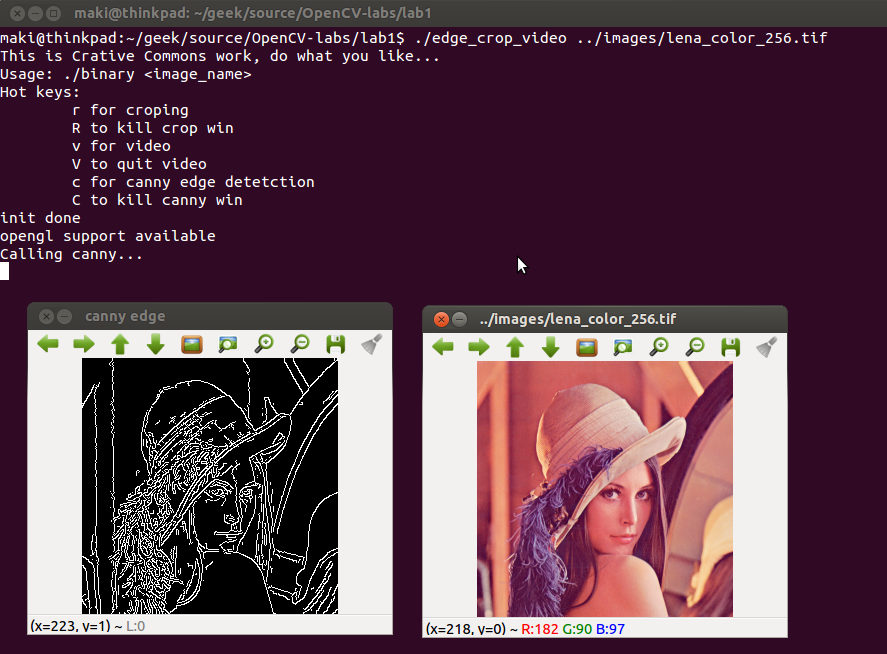
\includegraphics[scale=0.4]{images/lab1-01-edge.png}
\caption{Detekcija rubova}
\label{fig:lab1-01-edge}
\end{figure}

\newpage
\subsubsection{Rezanje slike}
Rezanje slike (engl. \textit{cropping}) je implementirano kroz poziv par
funkcija. Pritiskom na tipku \textbf{``r''} postavlja se
\textit{setMouseCallback} (funkcija koja konstantno poziva drugu
funkciju u slučaju micanja miša ili pritiska tipke) na funkciju
\textit{onMouse}. Funkciji \textit{onMouse} se također kroz
\textit{setMouseCallback} predaje i slika nad kojom je definiran
\textit{callback}.
\\

\begin{lstlisting}[language=C,caption={Rezanje slike}]
void onMouse( int event, int x, int y, int flags, void* param ) {
    Mat& image = *(Mat*) param;
    switch( event ) {
        case CV_EVENT_LBUTTONDOWN:
            drawing_box = true;
            box = Rect(x, y, 0, 0);
            break;
        case CV_EVENT_MOUSEMOVE: 
            if( drawing_box ) {
                box.width = x-box.x;
                box.height = y-box.y;
            } break;
        case CV_EVENT_LBUTTONUP: 
            drawing_box = false;
            if( box.width<0 ) {
                box.x+=box.width;
                box.width *= -1;
            }
            if( box.height<0 ) {
                box.y+=box.height;
                box.height*=-1;
            }
            draw_box( image, box );
            crop_image( image, box);
            break; } } 
void draw_box( Mat& img, Rect rect ){
    rectangle( img, rect.tl(), rect.br(), Scalar(0,0,255));
}
void crop_image( Mat& img, Rect rect ){
    Mat imgRoi = img(rect);
    namedWindow( "ImgROI", CV_WINDOW_AUTOSIZE );
    imshow( "ImgROI", imgRoi );
}
\end{lstlisting}

\begin{figure}[h]
\centering
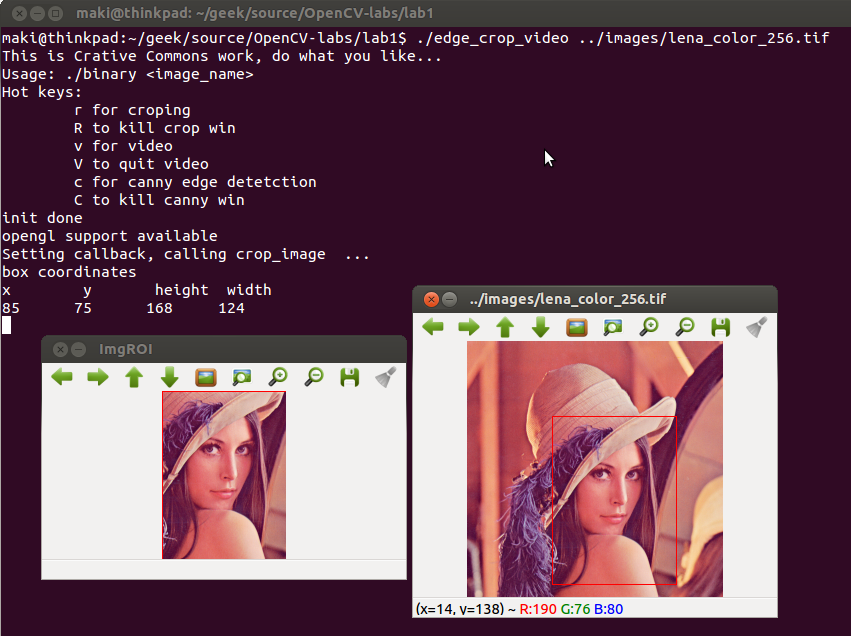
\includegraphics[scale=0.4]{images/lab1-02-crop.png}
\caption{Rezanje slike}
\label{fig:lab1-02-crop}
\end{figure}

\newpage
\subsubsection{Učitavanje videa}
Učitavanje videa ili kamere se događa nakon pritiska tipke
\textbf{``v''}. Time pozivamo funkciju \textit{init\_camera} koja
stvori objekt tipa \textit{VideoCapture}. Objekt prvo pokušu učitat
kameru ako ne uspije provjerava \textit{argv[2]} za drugim izvorom
kamere ili videa. Nakon toga u beskonačnoj petlji objekta se izvlači 
frame po frame i prikazuje u prozoru \textit{``camera``}.
\\
\begin{lstlisting}[language=C,caption={Učitavanje videa}]
void init_camera(){
    cout << "Starting camera mode... \n";
    VideoCapture cap(0);
    if( !cap.isOpened() ){
        cout << "isprobavam argv2 " 
            << global_argv[2] << endl;
        cap.open( global_argv[2] );
        if( !cap.isOpened() ){
            cerr << "fail i preko argv[2] \n"; 
            } 
        }
    while( 1 ){
        cap >> frame;
        if(!frame.data) break;
        namedWindow( "camera", CV_WINDOW_AUTOSIZE );
        imshow( "camera", frame );
        char c = waitKey(10);
        if( c == 'V' ){
            destroyWindow("camera");
            break; 
            } 
        } 
    }
\end{lstlisting}


\subsection{Zaključak}


Osnovni zadaci ove vježbe su bili upoznavanje s OpenCV bibliotekom,
podešavanje radne okoline i rješavanje par jednostavnijih zadataka.
Inicijalno podešavanje radne okoline je bitan zadatak jer o njemu ovisi
izvedba ove i budućih vježbi.
S OpenCV bibliotekom smo se upoznali kroz rješavanje zadataka.
Pisanje jednostavnog programa za detektiranje rubova na slici nam je
pružilo uvid u deklariranje \textit{Mat} varijabli za spremanje slika,
pozivanje OpenCV funkcija i prikazivanje tih slika.
Rješavanje problema rezanja slike nam je omogućilo upoznavanje s
\textit{mouseCallback} funkcijom koja je sastavni dio većine grafičkih
programa. Njeno razumjevanje je ključan dio za pisanje programa koji traže
interakciju s korisnikom. Osim toga naučili korisiti funkciju
\textit{rectangle} za crtanje pravokutnika na slici i definirati regiju
intersa na slici. 
Zadnji dio zadatka se odnosio na učitavanje videa. Osnovna stvar je bila
shvatiti kako \textit{VideoCapture} objekt funkcionira, te koje njegove
metode možemo korisiti.
Svi ovi zadaci su okosnice drugi programa. Detekcija rubova na slici s
kamere se može korisiti u programu koji detektira pokret.
Rezanje slike je poželjna funkcija svakog preglednika slika.



%\include{02_druga}

%\include{03_treca}

%\include{04_cetvrta}

%\include{05_peta}

%\include{06_sesta}
 
%\include{07_sedma}


\end{document}

